% !TEX root = hw7-answers-graded.tex
\chead{\textbf{Exercises week 7}}

\begin{document}
\flushleft\textbf{Topic: Marginalisation and interventions on Bayesian Networks}

\begin{enumerate}[label=7.\arabic*]
    \item \label{ex:binary_cbn} Consider the CBN with variables $V=\{X, Y, Z\}$, $J=\emptyset$, graph $G$ as given by Figure \ref{fig:one}, and Markov kernels given by
    \begin{align*}
        P(Z)      & = \mathrm{Bernoulli}\left(\frac{1}{3}\right),     \\
        P(X|Z)    & = \mathrm{Bernoulli}\left(\frac{1+Z}{3}\right),   \\
        P(Y|X, Z) & = \mathrm{Bernoulli}\left(\frac{1+X+Z}{4}\right).
    \end{align*}
    \begin{figure}[ht]
        \centering
        \begin{tikzpicture}[scale=1, transform shape]
            \node[ndout] (X) at (0, 0) {$X$};
            \node[ndout] (Y) at (2, 0) {$Y$};
            \node[ndout] (Z) at (1, 1) {$Z$};
            \draw[arout] (X) to (Y);
            \draw[arout] (Z) to (X);
            \draw[arout] (Z) to (Y);
        \end{tikzpicture}
        \caption{Causal graph $G$.}
        \label{fig:one}
    \end{figure}
    \begin{enumerate}
        \item Compute the difference $\alpha := E(Y \given X=1) - E(Y \given X=0)$.
        \item Give the graph and Markov kernels of the CBN after a hard intervention on $X$.
        \item Compute the \emph{average causal effect} $\beta := E(Y \given \doit(X=1)) - E(Y \given \doit(X=0))$.
        \item Let $X$ denote whether a patient takes a particular medicine, and let $Y$ denote whether the patient recovers. If a doctor measures an $n$-sample $(X_1, Y_1), ..., (X_n, Y_n)$, estimates $\alpha$ from the data and naively interprets it as the causal effect of the drug on the disease, which incorrect conclusion will they draw?
    \end{enumerate}
    \begin{ungradedsolution}
        \begin{enumerate}
            \item We have
            $$P(X=1) = P(X=1 | Z=0)P(Z=0) + P(X=1 | Z=1)P(Z=1) = \frac{1}{3}\cdot\frac{2}{3} + \frac{2}{3}\cdot\frac{1}{3} = \frac{4}{9}$$
            and
            \begin{align*}
                P(Z=0 | X=1) = P(X=1 | Z=0)P(Z=0)/P(X=1) = \frac{1}{3}\cdot\frac{2}{3} / \frac{4}{9} = \frac{1}{2}
            \end{align*}
            and $P(Z=1 | X=1) = \frac{1}{2}$, so
            \begin{align*}
                E(Y \given X=1) & = P(Y=1 \given Z=0, X=1)P(Z=0|X=1)                                         \\
                                & + P(Y=1 \given Z=1, X=1)P(Z=1|X=1)                                         \\
                                & = \frac{2}{4}\cdot\frac{1}{2} + \frac{3}{4}\cdot\frac{1}{2} = \frac{5}{8}.
            \end{align*}
            Similarly, $P(X=0) = \frac{5}{9}$ so
            \begin{align*}
                P(Z=0 | X=0) = P(X=0 | Z=0)P(Z=0)/P(X=0) = \frac{2}{3}\cdot\frac{2}{3} / \frac{5}{9} = \frac{4}{5}
            \end{align*}
            and $P(Z=1 | X=0) = \frac{1}{5}$, and
            \begin{align*}
                E(Y \given X=0) & = P(Y=1 \given Z=0, X=0)P(Z=0|X=0)                                          \\
                                & + P(Y=1 \given Z=1, X=0)P(Z=1|X=0)                                          \\
                                & = \frac{1}{4}\cdot\frac{4}{5} + \frac{2}{4}\cdot\frac{1}{5} = \frac{3}{10},
            \end{align*}
            so $\alpha = \frac{13}{40}\approx 0,325$.


            \item The intervention $\doit(X)$ gives the graph $G_{\doit(X)}$ as in Figure \ref{fig:two} and Markov kernels:
            \begin{align*}
                P(Z)     & = \mathrm{Bernoulli}\left(\frac{1}{3}\right),     \\
                % P(X)    & = \mathrm{Bernoulli}\left(\frac{1+Z}{3}\right),           \\
                P(Y|X,Z) & = \mathrm{Bernoulli}\left(\frac{1+X+Z}{4}\right).
            \end{align*}
            \begin{figure}[!ht]
                \centering
                \begin{tikzpicture}[scale=1, transform shape]
                    \node[ndint] (X) at (0, 0) {$X$};
                    \node[ndout] (Y) at (2, 0) {$Y$};
                    \node[ndout] (Z) at (1, 1) {$Z$};
                    \draw[arout] (X) to (Y);
                    % \draw[arout] (Z) to (X);
                    \draw[arout] (Z) to (Y);
                \end{tikzpicture}
                \caption{Causal graph $G_{\doit(X)}$.}
                \label{fig:two}
            \end{figure}

            \item
            We have
            \begin{align*}
                E(Y\given \doit(X=1)) & = P(Y=1 | X=1, Z=0)P(Z=0)                                                  \\
                                      & + P(Y=1 | X=1, Z=1)P(Z=1)                                                  \\
                                      & = \frac{2}{4}\cdot\frac{2}{3} + \frac{3}{4}\cdot\frac{1}{3} = \frac{7}{12}
            \end{align*}
            and
            \begin{align*}
                E(Y\given \doit(X=0)) & = P(Y=1 | X=0, Z=0)P(Z=0)                                                  \\
                                      & + P(Y=1 | X=0, Z=1)P(Z=1)                                                  \\
                                      & = \frac{1}{4}\cdot\frac{2}{3} + \frac{2}{4}\cdot\frac{1}{3} = \frac{4}{12}
            \end{align*}
            so $\beta = \frac{3}{12} \approx 0.25$.
            \item They overestimate the efficacy of the drug.
        \end{enumerate}
    \end{ungradedsolution}

    \item %($3 \times 1$ points)
    Consider the following CDMG $G$, where $A,H$ are input nodes:
    \begin{center}
        \begin{tikzpicture}[scale=1, transform shape]
            \node[ndout] (B) at (2, 0) {$B$};
            \node[ndout] (C) at (4, 0) {$C$};
            \node[ndout] (D) at (6, 0) {$D$};
            \node[ndout] (E) at (8, 0) {$E$};
            \node[ndout] (F) at (10, 0) {$F$};
            \node[ndint] (A) at (0, 0) {$A$};
            \node[ndint] (H) at (8, -2) {$H$};
            \draw[arint] (A) to (B);
            \draw[arout] (C) to (B);
            \draw[arout] (C) to (D);
            \draw[arout] (E) to (D);
            \draw[arout] (E) to (F);
            \draw[arint] (H) to (E);
        \end{tikzpicture}
    \end{center}
    \begin{enumerate}
        \item Is this graph cyclic? If not, give a topological ordering.
        % \item Do the following $d$-separations hold on graph $G$? Give a brief explanation for each answer. [Note, we write $C \Perp^d E \mid D$ for $\{C\} \Perp^d \{E\} \mid \{D\}$](4 $\times$ 1/4 pts)
        % \begin{enumerate}
        %   \item $\displaystyle  C \Perp^d E$
        %   \item $\displaystyle C \Perp^d E \mid D$
        %   \item $\displaystyle B \Perp^d D \mid \{A, H\}$
        %   \item $\displaystyle B \Perp^d D \mid \{C, A, H\}$
        % \end{enumerate}
        \item
        \begin{enumerate}
            \item Give $G^{\setminus C}$.
            \item Give ${G^{\setminus C}}^{\setminus E}$.
            \item Give ${{G^{\setminus C}}^{\setminus E}}^{\setminus D}$.
            \item Give $G^{\setminus E}$.
            \item Give ${G^{\setminus E}}^{\setminus C}$.
            \item Give $G^{\setminus \{C,E,D\}}$.
        \end{enumerate}
        Check that your answers agree with Lemma \ref*{marginalizations-commute}.
        % \item Does d-separation $\displaystyle B \Perp^d F \mid \{A, H\}$ hold on graphs $G, G^{\setminus \{C,E\}},G^{\setminus \{C,E,D\}}$? Explain without using Lemma 6.3.6 and check your answer with Lemma 6.3.6.
        \item
        \begin{enumerate}
            \item Give the graph $G_{\doit(\{D\})}$ after a hard intervention on $D$.
            \item Give the graph $G_{\doit(\{I_B\})}$ after a soft intervention on $B$.
            \item Give the graph $G_{\swig(E)}$ after a node-splitting intervention on $E$.
        \end{enumerate}
    \end{enumerate}

    \begin{ungradedsolution}
        \begin{enumerate}
            \item No: let $V := \{A, B, C, D, E, F, H\}$ and define the map $f:V\rightarrow \N$ as follows: $f(A) = 1, f(C) = 2, f(H) = 3, f(E) = 4, f(B) = 5, f(D) = 6, f(F) = 7$. This induces a topological ordering on $V$ via: $v < w \iff f(v) < f(w)$.
            \item
            \begin{enumerate}
                \item $G^{\setminus C}$:\\
                \begin{center}
                    \begin{tikzpicture}[scale=1, transform shape]
                        \node[ndout] (B) at (2, 0) {$B$};
                        \node[ndout] (D) at (6, 0) {$D$};
                        \node[ndout] (E) at (8, 0) {$E$};
                        \node[ndout] (F) at (10, 0) {$F$};
                        \node[ndint] (A) at (0, 0) {$A$};
                        \node[ndint] (H) at (8, -2) {$H$};
                        \draw[arint] (A) to (B);
                        \draw[arlat] (B) to (D);
                        \draw[arout] (E) to (D);
                        \draw[arout] (E) to (F);
                        \draw[arint] (H) to (E);
                    \end{tikzpicture}
                \end{center}
                \item ${G^{\setminus C}}^{\setminus E}$:\\
                \begin{center}
                    \begin{tikzpicture}[scale=1, transform shape]
                        \node[ndout] (B) at (2, 0) {$B$};
                        \node[ndout] (D) at (6, 0) {$D$};
                        \node[ndout] (F) at (10, 0) {$F$};
                        \node[ndint] (A) at (0, 0) {$A$};
                        \node[ndint] (H) at (8, -2) {$H$};
                        \draw[arint] (A) to (B);
                        \draw[arlat] (B) to (D);
                        \draw[arlat] (D) to (F);
                        \draw[arint] (H) to (D);
                        \draw[arint] (H) to (F);
                    \end{tikzpicture}
                \end{center}
                \item ${{G^{\setminus C}}^{\setminus E}}^{\setminus D}$: \\
                \begin{center}
                    \begin{tikzpicture}[scale=1, transform shape]
                        \node[ndout] (B) at (2, 0) {$B$};
                        \node[ndout] (F) at (10, 0) {$F$};
                        \node[ndint] (A) at (0, 0) {$A$};
                        \node[ndint] (H) at (8, -2) {$H$};
                        \draw[arint] (A) to (B);
                        \draw[arint] (H) to (F);
                    \end{tikzpicture}
                \end{center}
                \item $G^{\setminus E}$:\\
                \begin{center}
                    \begin{tikzpicture}[scale=1, transform shape]
                        \node[ndout] (B) at (2, 0) {$B$};
                        \node[ndout] (C) at (4, 0) {$C$};
                        \node[ndout] (D) at (6, 0) {$D$};
                        \node[ndout] (F) at (10, 0) {$F$};
                        \node[ndint] (A) at (0, 0) {$A$};
                        \node[ndint] (H) at (8, -2) {$H$};
                        \draw[arint] (A) to (B);
                        \draw[arout] (C) to (B);
                        \draw[arout] (C) to (D);
                        \draw[arout] (E) to (D);
                        \draw[arlat] (D) to (F);
                        \draw[arint] (H) to (D);
                        \draw[arint] (H) to (F);
                    \end{tikzpicture}
                \end{center}
                \item ${G^{\setminus E}}^{\setminus C}$:\\
                \begin{center}
                    \begin{tikzpicture}[scale=1, transform shape]
                        \node[ndout] (B) at (2, 0) {$B$};
                        \node[ndout] (D) at (6, 0) {$D$};
                        \node[ndout] (F) at (10, 0) {$F$};
                        \node[ndint] (A) at (0, 0) {$A$};
                        \node[ndint] (H) at (8, -2) {$H$};
                        \draw[arint] (A) to (B);
                        \draw[arlat] (B) to (D);
                        \draw[arlat] (D) to (F);
                        \draw[arint] (H) to (D);
                        \draw[arint] (H) to (F);
                    \end{tikzpicture}
                \end{center}
                \item $G^{\setminus \{C,E,D\}}$:\\
                \begin{center}
                    \begin{tikzpicture}[scale=1, transform shape]
                        \node[ndout] (B) at (2, 0) {$B$};
                        \node[ndout] (F) at (10, 0) {$F$};
                        \node[ndint] (A) at (0, 0) {$A$};
                        \node[ndint] (H) at (8, -2) {$H$};
                        \draw[arint] (A) to (B);
                        \draw[arint] (H) to (F);
                    \end{tikzpicture}
                \end{center}
            \end{enumerate}
            \item
            \begin{enumerate}
                \item $G_{\doit(\{D\})}$:
                \begin{center}
                    \begin{tikzpicture}[scale=1, transform shape]
                        \node[ndout] (B) at (2, 0) {$B$};
                        \node[ndout] (C) at (4, 0) {$C$};
                        \node[ndout] (E) at (8, 0) {$E$};
                        \node[ndout] (F) at (10, 0) {$F$};
                        \node[ndint] (A) at (0, 0) {$A$};
                        \node[ndint] (D) at (6, 0) {$D$};
                        \node[ndint] (H) at (8, -2) {$H$};
                        \draw[arint] (A) to (B);
                        \draw[arout] (C) to (B);
                        \draw[arout] (E) to (F);
                        \draw[arint] (H) to (E);
                    \end{tikzpicture}
                \end{center}
                \item $G_{\doit(\{I_B\})}$:
                \begin{center}
                    \begin{tikzpicture}[scale=1, transform shape]
                        \node[ndout] (B) at (2, 0) {$B$};
                        \node[ndout] (C) at (4, 0) {$C$};
                        \node[ndout] (D) at (6, 0) {$D$};
                        \node[ndout] (E) at (8, 0) {$E$};
                        \node[ndout] (F) at (10, 0) {$F$};
                        \node[ndint] (A) at (0, 0) {$A$};
                        \node[ndint] (I_B) at (2, -2) {$I_B$};
                        \node[ndint] (H) at (8, -2) {$H$};
                        \draw[arint] (A) to (B);
                        \draw[arint] (I_B) to (B);
                        \draw[arout] (C) to (B);
                        \draw[arout] (C) to (D);
                        \draw[arout] (E) to (D);
                        \draw[arout] (E) to (F);
                        \draw[arint] (H) to (E);
                    \end{tikzpicture}
                \end{center}
                \item $G_{\swig(E)}$:
                \begin{center}
                    \begin{tikzpicture}[scale=1, transform shape]
                        \node[ndout] (B) at (2, 0) {$B$};
                        \node[ndout] (C) at (4, 0) {$C$};
                        \node[ndout] (D) at (6, 0) {$D$};
                        \node[ndout] (Eo) at (8,-.4) {$E^o$};
                        \node[ndout] (F) at (10, 0) {$F$};
                        \node[ndint] (A) at (0, 0) {$A$};
                        \node[ndint] (Ei) at (8,0.4) {$E^i$};
                        \node[ndint] (H) at (8, -2) {$H$};
                        \draw[arint] (A) to (B);
                        \draw[arout] (C) to (B);
                        \draw[arout] (C) to (D);
                        \draw[arout] (Ei) to (D);
                        \draw[arout] (Ei) to (F);
                        \draw[arint] (H) to (Eo);
                    \end{tikzpicture}
                \end{center}
            \end{enumerate}
        \end{enumerate}
    \end{ungradedsolution}

    \item %($2 + 1 + 1 + 1$ points)
    The following problem is inspired by the television game show \emph{Let's make a
        deal} that was presented by Monty Hall in the eighties. Suppose you're
    participating in this show. You see three closed doors, and Monty tells you
    that behind one of those three doors, there is a car for you to win, but behind
    the other two doors, there are goats. Let us assume you would have a
    strong preference to win a car instead of a goat.
    Monty asks you to choose a door. After you tell him your choice, Monty (who
    knows where the car is hidden) opens one of the two other doors that you didn't
    choose, always picking one such that there is a goat behind that door. Then he asks you
    whether you would like to keep your original choice (\textbf{\emph{stick}}), or whether you would
    rather choose another door (\textbf{\emph{switch}}). He will open the door of your final choice and you
    will win whatever is behind that door.

    \centerline{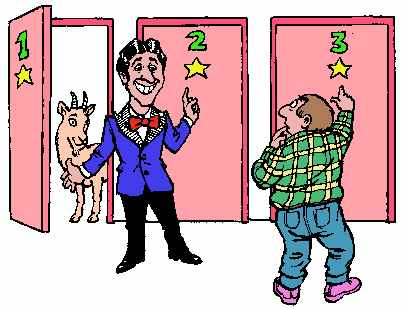
\includegraphics[width=5cm]{montyhall.jpg}}

    We use a Causal Bayesian Network to model this problem.
    \begin{enumerate}
        \item Define a L-CBN (see Definition \ref*{def:il-cbn}) that fits with the story.
        % TODO 2023: modeled form Monty's perspecitve (to prevent students to model L as an input node)/
        Use the following variables:\\[0.5\baselineskip]
        \centerline{
            \begin{tabular}{ll}
                $C$: & initial choice (``choice'')                                               \\
                $L$: & door behind which the prize is hidden (``location'')                      \\
                $D$: & door opened after you made your initial choice (``door'')                 \\
                $F$: & final choice after choosing to switch (or not)                            \\
                $I$: & node representing our strategy, $0$ if we do not switch, $1$ if we switch \\
                $O$: & what is behind the opened door of the final choice (``observation'')      \\
            \end{tabular}}
        So give the causal graph, clearly indicate the codomain of each variable, which variables are observed, unobserved (at the moment just before you make your final choice) and input nodes. Explain these modeling choices. Also, for each output node in the causal graph, provide the discrete Markov kernel corresponding to the story.
        \item Calculate the probability of winning given $I=1$ and $I=0$.

        \emph{Hint: You may use the fact that the problem is symmetric, and fix the initially chosen door to $1$.}
    \end{enumerate}
    Now let us change the story slightly. Suppose that before Monty can actually open a door (to show you that there is a goat behind that door), an earthquake intervenes and happens to open one of the two doors that you didn't choose initially, and you observe that there is a goat behind that door. Undisturbed by the earthquake, Monty thinks ``the show must go on!'' and proceeds by asking you what your final choice is.
    \begin{enumerate}[resume*]
        \item The earthquake intervention changes the causal Bayesian network. Draw the intervened causal graph (where we consider the earthquake as independently at random making a hard intervention on $D$).
        % TODO 2023: independently at random performing a hard intervening doesn't make sense, as we don't assume a distribution on input variables. We can better say that D is now Uniform({1, 2, 3}) independent of C and L, and add a selection variable S=1 iff D\neq C and D\neq L, and only consider the distributions conditioned on S=1.
        What is now our probability of winning given $I=1$ and $I=0$?
        \item Write four simulation programs (in either Python, R, Matlab or Julia): one where we \emph{stick}, one where we \emph{switch} after Monty opens a door, one where we \emph{stick}, and one where we \emph{switch} after an earthquake opens a door (where we condition on the door opened not being a car, i.e.\ we throw away samples where the earthquake happened to open the door with the car).
        % TODO 2023: also throw away the samples where the earthquake happened to open the door of the candidates initial choice.
        Explicitly model the generative process of the game. Use these simulations to estimate the win probability of each scenario using at least 1000 samples.

        \emph{Please also upload the .R/.py/.m/.jl file when submitting your assignment.}
    \end{enumerate}

    \begin{gradedsolution}
        \begin{figure}[ht]
            \begin{subfigure}[]{0.45\textwidth}
                \centering
                \begin{tikzpicture}[scale=1, transform shape]
                    \node[ndout] (L) at (4,0) {$L$};
                    \node[ndout] (D) at (2,0) {$D$};
                    \node[ndout] (F) at (2,-2) {$F$};
                    \node[ndout] (O) at (4,-2) {$O$};
                    \node[ndint] (C) at (0,0) {$C$};
                    \node[ndint] (I) at (0,-2) {$I$};
                    \draw[arout] (C) to (D);
                    \draw[arout] (L) to (D);
                    \draw[arout] (C) to (F);
                    \draw[arout] (D) to (F);
                    \draw[arout] (I) to (F);
                    \draw[arout] (F) to (O);
                    \draw[arout] (L) to (O);
                \end{tikzpicture}
                \caption{}
                \label{fig:mh}
            \end{subfigure}
            \begin{subfigure}[]{0.45\textwidth}
                \centering
                \begin{tikzpicture}[scale=1, transform shape]
                    \node[ndout] (L) at (4,0) {$L$};
                    \node[ndout] (F) at (2,-2) {$F$};
                    \node[ndout] (O) at (4,-2) {$O$};
                    \node[ndint] (C) at (0,0) {$C$};
                    \node[ndint] (D) at (2,0) {$D$};
                    \node[ndint] (I) at (0,-2) {$I$};
                    \draw[arout] (C) to (F);
                    \draw[arout] (D) to (F);
                    \draw[arout] (I) to (F);
                    \draw[arout] (F) to (O);
                    \draw[arout] (L) to (O);
                \end{tikzpicture}
                \caption{}
                \label{fig:mh2}
            \end{subfigure}
        \end{figure}
        \begin{enumerate}
            \item \points{1} We have represented a possible graph for this problem in figure \ref{fig:mh}. The codomains of all variables are given by $\{1,2,3\}$, except for $I$ and $O$ which take values in $\{0,1\}$ (where a $1$ for $O$ represents winning a car). $L, F$ and $O$ are unobserved variables (right before making the final decision). Note that representing both situations in a single graph loses some information compared to modeling two separate graphs: for example there is no arrow from $D$ to $F$ if $I=0$. In this graph we clearly see that knowledge about $L$ might influence our final choice through $D$.

            The Markov kernels that define the Bayesian network are:
            \begin{align*}
                P(L)                & = \mathrm{Unif}(\{1, 2, 3\})                                             \\
                P(D|C=c, L=\ell)    & = \begin{cases}
                                            \mathrm{Unif}(\{1, 2, 3\}\setminus \{c\}) & \text{if $c=\ell$}    \\
                                            \delta_{\{1, 2, 3\}\setminus \{c, \ell\}} & \text{if $c\neq\ell$}
                                        \end{cases}      \\
                P(F|I=i, C=c, D=d)  & = \begin{cases}
                                            \delta_{\{c\}}                         & \text{if $i=0$}               \\
                                            \delta_{\{1, 2, 3\}\setminus \{c, d\}} & \text{if $i=1$ and $c\neq d$} \\
                                            \text{arbitrary}                       & \text{if $i=1$ and $c= d$}
                                        \end{cases} \\
                P(O=1 |F=f, L=\ell) & = \I_{\{\ell\}}(f)
            \end{align*}

            % We see that $L$ has a discrete uniform distributions on its domain. We define the Markov kernel $P(D|C, L)$ by two cases
            % \begin{itemize}
            %   \item If $c=l$ then it is the uniform distribution on $\{1,2,3\} \setminus \{c\}$.
            %   \item If $c \neq l$, then $P(D=d|C=c, L=l) = 1 - \delta_{\{c,l\}}(d)$.
            % \end{itemize}
            % Similarly for the Markov kernel $P(F|I, C, D)$ we distinguish cases:
            % \begin{itemize}
            %   \item If $I=0$, then $P(F=f|I=0, C=c, D=d) = \delta_{\{c\}}(f)$.
            %   \item If $I=1$, then by the generative process we only have to concern ourselves with the case where $c \neq d$, in which case $P(F=f|I=0, C=c, D=d) = 1 - \delta_{\{c,d\}}(f)$. If $c = d$ we may define the Markov kernel as some arbitrary distribution over $F$.
            % \end{itemize}
            % Finally, $P(O \given F, L)$ is defined by the probability mass function $P(O=1 \given F=f, L=l) = \delta_{\{l\}}(f)$.

            \item \points{1}
            Formally, for $i\in\{0,1\}$ we are interested in the quantity
            \begin{equation*}
                P(O=1|I=i, C=1) = P(O=1 | F, L)\circ P(F|I=i, C=1, D)\circ P(D|C=1, L)\circ P(L),
            \end{equation*}
            where we arbitrarily picked $C=1$ following the hint from the exercise. This can be explicitly calculated by writing the above expression as a repeated sum over possible values of $F, D$ and $L$, and using the definitions of the Markov kernels as given in part a).

            A more intuitive argumentation would be that if we set $I=0$ and pick $C=1$, we can only win if $L=1$, so
            \begin{equation*}
                P(O =1 \given I=0, C=1) = P(L=1) = \frac{1}{3}.
            \end{equation*}
            If we set $I=1$ and pick $C=1$, we can only win if $L\neq 1$, in which case $F=L$ and we win the game, so
            \begin{equation*}
                P(O =1 \given I=1, C=1) = P(L\neq 1) = \frac{2}{3}.
            \end{equation*}

            \item \points{1}
            The graph after earthquake intervention is shown in figure \ref{fig:mh2}.
            We are asked to calculate the quantity $P(O=1|I=i, C=1, D=d)$ for $d\in\{2, 3\}$ and $i\in\{0,1\}$:
            \begin{align*}
                P(O=1|I=0, C=1, D=2) & = P(L=1|L\neq 2) = \left.\frac{1}{3}\middle/ \frac{2}{3} = \frac{1}{2}\right.   \\
                P(O=1|I=1, C=1, D=2) & = P(L=3|L\neq 2) = \left.\frac{1}{3} \middle/ \frac{2}{3} = \frac{1}{2}\right.,
            \end{align*}
            and using symmetry in $D$ we conclude that $P(O=1|I=0, C=1, D=3) = P(O=1|I=1, C=1, D=3) = 1/2$ as well.

            % It is clear since $F$ has to match $L$ and $L$ is independently drawn, that the win probability is the same for all strategies, i.e.\ the probability of winning is $1/2$ since there are now $2$ doors to choose from. Conditioning on $D$ does not open a path.
            \item \points{2} An example of an \emph{R} script is given as follows:
        \end{enumerate}
    \end{gradedsolution}

    \textcolor{red}{\textbf{!!! SOLUTION: !!!}}
    \begin{lstlisting}[language=R]
      # R code for Monty Hall problem normal variant
      #############################################
      initial_choice <- sample(c(1,2,3),1000, replace=TRUE)
      car <- sample(c(1,2,3),1000, replace=TRUE)
      
      # Define a function that given a combination of initial_choice 
      # and car samples door correctly
      f1 <- function(ic,ca) {
          space <- c(1,2,3)
          if (ic == ca) {
              return(sample(space[space != ic],1, replace=TRUE))
          } else {
              return(space[space != ic & space != ca])
          }
      }
      # Apply this to the combination of initial_choice and car vectors
      door <- mapply(f1, initial_choice,car)
      
      # Switch or do not switch:
      final_choice_stick <- initial_choice
      final_choice_switch <- 1*(initial_choice != 1 & door != 1) + 
                              2*(initial_choice != 2 & door != 2) + 
                              3*(initial_choice != 3 & door != 3)
      
      # Calculate win probabilities
      print(mean((final_choice_switch == car)))
      print(mean((final_choice_stick == car)))
  \end{lstlisting}

    \begin{lstlisting}[language=R]
      # R code for Monty Hall problem earthquake intervention
      #######################################################
      initial_choice <- sample(c(1,2,3),5000, replace=TRUE)
      car <- sample(c(1,2,3),5000, replace=TRUE)
      door <- sample(c(1,2,3),5000, replace=TRUE)
      
      mask <- (door != initial_choice) & (door != car) 
      
      final_choice_switch <- 1*(initial_choice != 1 & door != 1) + 
                          2*(initial_choice != 2 & door != 2) + 
                          3*(initial_choice != 3 & door != 3)
      
      final_choice_stick <- initial_choice
      
      print(mean((final_choice_switch == car)[mask]))
      print(mean((final_choice_stick == car)[mask]))
    \end{lstlisting}

\end{enumerate}

% TODO 2023:
% \textcolor{red}{Update 05/04/2023, PB: }
% During todays TA session, it seemed that in question 2c) modelling the earthquake as a hard intervention is not very satisfactory, since in the story it says that ''an earthquake intervenes and happens to open one of the two doors that you didn't choose initially, and you observe that there is a goat behind that door''.

% The causal graph in Figure \ref{fig:mh2} doesn't really tell the story correctly. Consider $P(O=1|I=0, C=1, L=2, D=d)$, then the story implies that we can only consider $P(O=1|I=0, C=1, L=2, D=3)$ and not $P(O=1|I=0, C=1, L=2, D=2)$, as the earthquake may not open the door that has a car behind it. We were discussing about whether there should be an arrow from $L$ to $D$ to represent this restriction. I first suggested that the story `just restricts the values of $d$ that can be considered as input', but this is also not very satisfactory, as this depends on the value of $L$. Eventually I found that perhaps a better model for this story is as depicted in Figure \ref{fig:mh3}, with $S=1$ iff $D\neq C$ and $D\neq L$, and where we only consider the distribution conditioned on $S=1$. This is also in line with the way this is simulated in question d), i.e.\ the samples where the earthquake opens the door with the car behind it are thrown out.
% \begin{figure}[ht]
%   \centering
%   \begin{tikzpicture}[scale=1, transform shape]
%     \node[ndout] (L) at (4,0) {$L$};
%     \node[ndout] (F) at (2,-2) {$F$};
%     \node[ndout] (O) at (4,-2) {$O$};
%     \node[ndint] (C) at (0,0) {$C$};
%     \node[ndout] (D) at (2,0) {$D$};
%     \node[ndout] (S) at (2,2) {$S$};
%     \node[ndint] (I) at (0,-2) {$I$};
%     \draw[arout] (C) to (F);
%     \draw[arout] (D) to (F);
%     \draw[arout] (I) to (F);
%     \draw[arout] (F) to (O);
%     \draw[arout] (L) to (O);
%     \draw[arout] (C) to (S);
%     \draw[arout] (D) to (S);
%     \draw[arout] (L) to (S);
%   \end{tikzpicture}
%   \caption{}
%   \label{fig:mh3}
% \end{figure}
